%
% Copyright (c) 2017 Intel Corporation
%
% Permission is hereby granted, free of charge, to any person obtaining a copy
% of this software and associated documentation files (the "Software"), to
% deal in the Software without restriction, including without limitation the
% rights to use, copy, modify, merge, publish, distribute, sublicense, and/or
% sell copies of the Software, and to permit persons to whom the Software is
% furnished to do so, subject to the following conditions:
%
% The above copyright notice and this permission notice shall be included in
% all copies or substantial portions of the Software.
%
% THE SOFTWARE IS PROVIDED "AS IS", WITHOUT WARRANTY OF ANY KIND, EXPRESS OR
% IMPLIED, INCLUDING BUT NOT LIMITED TO THE WARRANTIES OF MERCHANTABILITY,
% FITNESS FOR A PARTICULAR PURPOSE AND NONINFRINGEMENT. IN NO EVENT SHALL THE
% AUTHORS OR COPYRIGHT HOLDERS BE LIABLE FOR ANY CLAIM, DAMAGES OR OTHER
% LIABILITY, WHETHER IN AN ACTION OF CONTRACT, TORT OR OTHERWISE, ARISING
% FROM, OUT OF OR IN CONNECTION WITH THE SOFTWARE OR THE USE OR OTHER DEALINGS
% IN THE SOFTWARE.
%

\newcommand{\repoTopPath}{../../..}
\newcommand{\commonPreamblePath}{\repoTopPath/common/latex/common_preamble.tex}
\input \commonPreamblePath

%----BEGIN TYPESETTING----------------------------------------------------------
\begin{document}
\sffamily

% create our own title area rather than \begin{titlepage} or \maketitle
\begin{center}
\let\savethefootnote\thefootnote
\let\thefootnote\relax\footnote{Intel, and Quartus are trademarks of Intel Corporation or its subsidiaries in the U.S. and/or other countries.}
\addtocounter{footnote}{-1}
\let\thefootnote\savethefootnote
\hspace{-1em}
\let\savethefootnote\thefootnote
\let\thefootnote\relax\footnote{Other names and brands may be claimed as the property of others.}
\addtocounter{footnote}{-1}
\let\thefootnote\savethefootnote
\hspace{-1em}
\LARGE{Interacting with FPGA Designs using Linux\textsuperscript{*}}\\[1em]
\end{center}

\begin{flushleft}
\normalsize{PDF created: \today}\\
\normalsize{Validated using tools release: \TheToolsReleaseVersion}
\end{flushleft}

% make an entry in the PDF bookmarks for the TOC
\pdfbookmark[0]{Contents}{sumario_label}
% insert the default TOC format
\tableofcontents

%----NEW SECTION DEFINITION-----------------------------------------------------
\section*{Overview}
% must manually add TOC reference for unnumbered section
\addcontentsline{toc}{section}{Overview}
%----NEW SECTION DEFINITION-----------------------------------------------------

\begin{flushleft}
\noindent
This tutorial demonstrates how to use various Linux capabilities to interact with the hardware modules instantiated in an FPGA design from the HPS processor.  This Linux tutorial is based on the FPGA design created in a prior tutorial \textquote{My First HPS System}.  In that tutorial you create this Qsys system:

\begin{figure}[H]
\centering
% screen shots report a density of 37.8 PixelsPerCentimeter when actual resolution
% is more like 56 PixelsPerCentimeter, so the scaling factor for 1:1 is 0.675
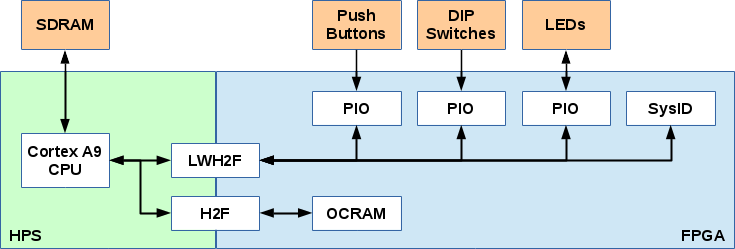
\includegraphics[scale=0.90]{hps_block_diagram}
\caption{HPS System Block Diagram}
\label{fig:hps_block_diagram}
\end{figure}

In this tutorial we will demonstrate how you can interact with the Qsys system in the FPGA through the HPS-to-FPGA bridges provided on the HPS core, reading and writing to the slave peripherals they are connected to.  We demonstrate the \emph{devmem} and \emph{devmem2} programs that can peek and poke at the FPGA peripherals.  We also demonstrate how to build a Linux application to interact with those same soft IP peripherals.  Finally we demonstrate how to use a number of \emph{sysfs} capabilities provided by existing device drivers for the FPGA based peripherals which we will enable with a \emph{device tree overlay}.

\end{flushleft}

%----NEW SECTION DEFINITION-----------------------------------------------------
\section*{Prerequisites}
% must manually add TOC reference for unnumbered section
\addcontentsline{toc}{section}{Prerequisites}
%----NEW SECTION DEFINITION-----------------------------------------------------

\begin{flushleft}
\noindent
The following are required:

\begin{itemize}

\item Linux development host PC with internet connection and serial terminal emulator
\item Completed Intel\textsuperscript{\textregistered} Quartus\textsuperscript{\textregistered} software project from \textquote{My First HPS System}
\begin{itemize}
\item Either follow the tutorial steps presented \href{\TheReleasesURL/writeup_MyFirstHPSSystem.pdf}{\underline{here}}.
\item Or, obtain the prebuilt output required from that tutorial \hyperlink{blinkArchive}{\underline{here}}
\end{itemize}
\item Terasic DE-10 Nano SD Card Image Archive: \small \MySDIMAGETGZ \normalsize
\begin{itemize}
\item You can download the archive from this location \href{https://downloadcenter.intel.com/download/26687/Downloads-for-the-Terasic-DE10-Nano-Kit-Featuring-an-Intel-Cyclone-V-FPGA-SoC}{https://\allowbreak downloadcenter.\allowbreak intel.\allowbreak com/\allowbreak download/\allowbreak 26687/\allowbreak Downloads-\allowbreak for-\allowbreak the-\allowbreak Terasic-\allowbreak DE10-\allowbreak Nano-\allowbreak Kit-\allowbreak Featuring-\allowbreak an-\allowbreak Intel-\allowbreak Cyclone-\allowbreak V-\allowbreak FPGA-\allowbreak SoC}
\end{itemize}
\item Terasic DE10-Nano board
\item MicroSD\textsuperscript{*} card for Terasic DE10-Nano
\item MicroSD card adapter for host PC if necessary
\item Power supply for Terasic DE10-Nano
\item Mini USB cable to connect Terasic DE10-Nano UART console port with PC

\end{itemize}

Notes:

\begin{itemize}

\item The SD card image archive and the \textbf{blink} hardware project from the \textquote{My First HPS System} tutorial are assumed to be stored in the \textbf{\$DE10\_NANO} folder on the host PC. Make sure you define this environment variable to point at the location where these files are stored. For instance, if you store these files in your \textbf{HOME} directory, in a directory called \textbf{de10-nano}, you can define the environment variable like this:

\begin{minted}[
	bgcolor=MyMintedBGColor,
	escapeinside=++
]{text}

+\$+ export DE10_NANO=+\textasciitilde+/de10-nano

\end{minted}

\item The following files from the \textbf{blink} hardware project are used by this guide:

\begin{itemize}

\item \texttt{blink/output\_files/blink.rbf} - for configuring the FPGA from U-Boot

\item \texttt{blink/qsys\_headers/hps\_0\_arm\_a9\_0.h} - for details about IP addresses inside the FPGA fabric

\end{itemize}

\item \hypertarget{blinkArchive}{If} you need the prebuilt files from the \textbf{blink} hardware project, you can download them to your local file system \href{\TheReleasesURL/blink_for_uboot.zip}{\underline{here}}.  Save the ZIP archive file to this location, \textbf{\$DE10\_NANO/}, the location stored in the environment variable suggested in the note above.  After you have stored the archive you can extract the contents like this:

%\item \hypertarget{blinkArchive}{If} you need the prebuilt files from the \textbf{blink} hardware project, you can extract this PDF attachment to your local file system: \textattachfile[
%	color=0.0 0.678 0.937,
%	mimetype=application/zip,
%	description={ZIP Archvie File: blink.zip}
%]{../../writeup_u-boot/blink_archive/blink.zip}{\textbf{blink.zip}}. Right click on the PDF attachment link and your PDF reader should present a pop-up menu with an option to save the attachment to your local file system.  Save the ZIP archive file to this location, \textbf{\$DE10\_NANO/}, the location stored in the environment variable suggested in the note above.  After you have stored the archive you can extract the contents like this:

\begin{minted}[
	bgcolor=MyMintedBGColor,
	escapeinside=++
]{text}

+\$+ cd +\$+DE10_NANO
+\$+ unzip blink_for_uboot.zip

\end{minted}

\item Throughout this guide, filenames and parameters that can change based on the latest release filenames or host computer configuration are marked in \textcolor{red}{red}.  You may need to change those values based on your specific environment and the version that you are using.

\end{itemize}

\end{flushleft}

%----NEW SECTION DEFINITION-----------------------------------------------------
\section*{Preparing the Terasic DE10-Nano Board}
% must manually add TOC reference for unnumbered section
\addcontentsline{toc}{section}{Preparing the Terasic DE10-Nano Board}
%----NEW SECTION DEFINITION-----------------------------------------------------

\begin{flushleft}
\noindent

This section describes how to prepare the Terasic DE10-Nano board for use in this tutorial.

\begin{enumerate}[
	label=\textbf{Step \arabic*.},
	leftmargin=*,
	widest={00},
	align=left]

\item Remove the microSD card from your Terasic DE10-Nano board and insert it into your host PC using an appropriate adapter if necessary.

\newpage

\item Extract the SD card image from the archive by running the following command:

\begin{minted}[
	bgcolor=MyMintedBGColor,
	escapeinside=++
]{text}

+\$+ cd +\$+DE10_NANO
+\$+ tar xf +\MySDIMAGETGZ+

\end{minted}

\item Write the SD card image to the microSD card using the \textbf{dd} command:

\begin{minted}[
	bgcolor=MyMintedBGColor,
	escapeinside=++
]{text}

+\$+ sudo dd if=+\MySDIMAGE+ of=+\textcolor{red}{/dev/sdx}+ bs=16M

\end{minted}

After the SD image is copied to your microSD card some systems may automatically detect the new partitions that have been copied onto the microSD card and you will not have to manually probe them.  If you do need to manually probe the partitions to get them to appear in your environment properly, you can do it like this:

\begin{minted}[
	bgcolor=MyMintedBGColor,
	escapeinside=++
]{text}

+\$+ sudo partprobe +\textcolor{red}{/dev/sdx}+

\end{minted}

\item Download the Linux examples archive \href{\TheReleasesURL/linux_examples.zip}{\underline{here}}.  Save the ZIP archive file to this location \textbf{\$DE10\_NANO/linux\_examples.zip}.

%\item Extract this PDF attachment to your local file system: \textattachfile[
%	color=0.0 0.678 0.937,
%	mimetype=application/zip,
%	description={ZIP Archive File: linux\_examples.zip}
%]{../linux_examples_archive/linux_examples.zip}{\textbf{linux\_examples.zip}}.  Right click on the PDF attachment link and your PDF reader should present a pop-up menu with an option to save the attachment to your local file system.  Save the ZIP archive file to this location \textbf{\$DE10\_NANO/}.

\item Download the source code for the \emph{devmem} utility:

\begin{minted}[
	fontsize=\small,
	bgcolor=MyMintedBGColor,
	escapeinside=||
]{text}

# you can do this two different ways, use git to clone the repo and extract the
# desired file, or download the repo archive and extract the desired file

# using git you can do this:
|\$| git clone https://gfiber.googlesource.com/vendor/opensource/toolbox
|\$| cp toolbox/devmem.c .
|\$| rm -rf toolbox

# or you can download the repo archive like this:
|\$| wget https://gfiber.googlesource.com/vendor/opensource/toolbox/+archive/master.tar.gz
|\$| tar xf master.tar.gz devmem.c
|\$| rm master.tar.gz

\end{minted}

\item Download the source code for the \emph{devmem2} utility:

\begin{minted}[
	bgcolor=MyMintedBGColor,
	escapeinside=++
]{text}

+\$+ wget http://free-electrons.com/pub/mirror/devmem2.c

\end{minted}

\item Mount the FAT partition of the microSD card on the host PC, and copy the required files to it. Depending on your host PC configuration, the mounting may happen automatically.  The FAT partition is partition 1 on the microSD card.  The instructions below assume manual mounting is needed:

\begin{minted}[
	bgcolor=MyMintedBGColor,
	escapeinside=++
]{text}

# create a directory in +\$+DE10_NANO to use as a mount point
+\$+ mkdir sdcard

# mount partition 1 of the microSD card, this is the FAT partition
+\$+ sudo mount +\textcolor{red}{/dev/sdx}+1 sdcard

# copy the required files onto the FAT partition
+\$+ sudo cp +\$+DE10_NANO/blink/output_files/blink.rbf sdcard/
+\$+ sudo cp +\$+DE10_NANO/blink/qsys_headers/hps_0_arm_a9_0.h sdcard/
+\$+ sudo cp +\$+DE10_NANO/devmem.c sdcard/
+\$+ sudo cp +\$+DE10_NANO/devmem2.c sdcard/
+\$+ sudo cp +\$+DE10_NANO/linux_examples.zip sdcard/

# unmount the FAT partition
+\$+ sudo umount sdcard
+\$+ sudo sync

\end{minted}

\item Remove the microSD card from your host PC and insert it into the Terasic DE10-Nano board.

\item Configure the Terasic DE10-Nano dip switch block \textbf{SW10} (highlighted in red below) to these positions from left to right as viewed with the board oriented as shown in the image below: \texttt{UP-DOWN-UP-DOWN-UP-UP}

\begin{figure}[H]
\centering
% screen shots report a density of 37.8 PixelsPerCentimeter when actual resolution
% is more like 56 PixelsPerCentimeter, so the scaling factor for 1:1 is 0.675
\scriptsize{Image used with permission from Terasic Technologies Inc.}
\newline
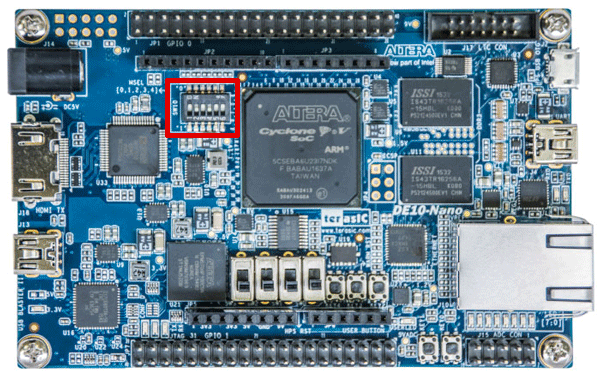
\includegraphics[scale=0.675]{de10-nano_sw10}
\caption{SW10 Configuration}
\label{fig:de10-nano_sw10}
\end{figure}

\item Plug a mini USB cable into the Terasic DE10-Nano UART console connector (highlighted in red below),  then plug the other end of the USB cable into your host PC.

\begin{figure}[H]
\centering
% screen shots report a density of 37.8 PixelsPerCentimeter when actual resolution
% is more like 56 PixelsPerCentimeter, so the scaling factor for 1:1 is 0.675
\scriptsize{Image used with permission from Terasic Technologies Inc.}
\newline
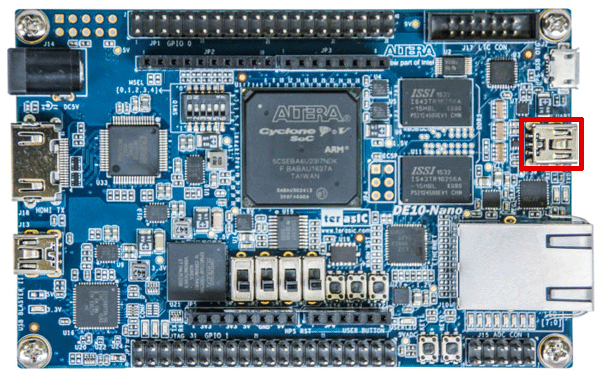
\includegraphics[scale=0.675]{de10-nano_uart}
\caption{UART Console Connector on Terasic DE10-Nano Board}
\label{fig:de10-nano_uart}
\end{figure}

\item On the host PC, start a serial terminal (for example minicom, or putty) and connect to the serial port corresponding to the Terasic DE10-Nano UART console using the serial communication settings: \texttt{115,200-8-N-1}.

\item Power the Terasic DE10-Nano board by inserting the power supply cord into the power connector (highlighted in red below).

\begin{figure}[H]
\centering
% screen shots report a density of 37.8 PixelsPerCentimeter when actual resolution
% is more like 56 PixelsPerCentimeter, so the scaling factor for 1:1 is 0.675
\scriptsize{Image used with permission from Terasic Technologies Inc.}
\newline
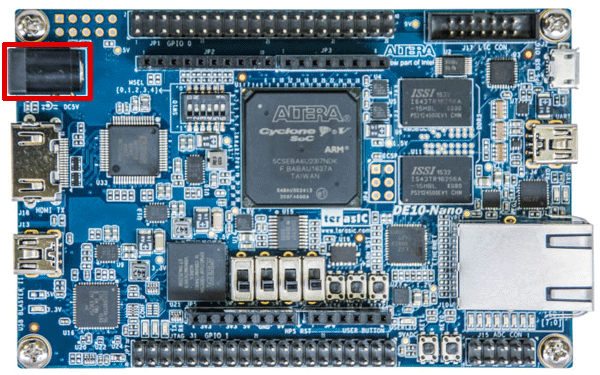
\includegraphics[scale=0.675]{de10-nano_pwr}
\caption{Power Connector on Terasic DE10-Nano Board}
\label{fig:de10-nano_pwr}
\end{figure}

\item In the serial terminal, you should observe the boot messages as U-Boot starts and configures the FPGA and boots the Linux kernel.  After a few seconds you will see the Angstrom logo scroll into view and a login prompt.  You may also see some lingering boot messages related to the CRDA update that the cfg80211 driver is attempting to perform, this will eventually timeout and stop.

\begin{minted}[
	bgcolor=MyMintedBGColor,
	escapeinside=++
]{text}

[   31.907948] cfg80211: Calling CRDA to update world regulatory domain
[   35.067904] cfg80211: Exceeded CRDA call max attempts. Not calling CRDA

\end{minted}

If your login prompt was overwritten by the lingering boot message output, press return to get a clean login prompt again.  Login with the username \textbf{root} and empty password (simply press the \textbf{enter} key for the password).

\begin{minted}[
	bgcolor=MyMintedBGColor,
	escapeinside=++
]{text}

.---O---.
|       |                  .-.           o o
|   |   |-----.-----.-----.| |   .----..-----.-----.
|       |     | __  |  ---'| '--.|  .-'|     |     |
|   |   |  |  |     |---  ||  --'|  |  |  '  | | | |
'---'---'--'--'--.  |-----''----''--'  '-----'-'-'-'
                -'  |
                '---'

The Angstrom Distribution de10-nano ttyS0

Angstrom v2016.12 - Kernel 4.1.33-ltsi-altera

de10-nano login: root
Password: +\textcolor{red}{<the password is NULL so just press ENTER>}+
root@de10-nano:~#

\end{minted}

\item We need to disable some of the default functionality that the standard Terasic DE10-Nano SD card image assumes.  Primarily we need to disable all of the functionality that depends on the default FPGA image so that we can load our \textbf{blink.rbf} instead.  There are five services that get started in the systemd init environment which require the default FPGA image to be available, we will disable those services with the following commands:

\begin{minted}[
	bgcolor=MyMintedBGColor,
	escapeinside=++
]{text}

# configure the linux environment so we can run our custom blink.rbf instead of
# the default RBF image.  The following five services must be disabled:
+\textbf{root@de10-nano:~#}+ systemctl disable de10-nano-fpga-leds.service
+\textbf{root@de10-nano:~#}+ systemctl disable de10-nano-synergy-init.service
+\textbf{root@de10-nano:~#}+ systemctl disable de10-nano-fftsw-init.service
+\textbf{root@de10-nano:~#}+ systemctl disable de10-nano-fpga-init.service
+\textbf{root@de10-nano:~#}+ systemctl disable de10-nano-xfce-init.service

\end{minted}

If you ever want to enable the Linux environment to run with the default RBF image again, you can simply re-enable those five services like this:

\begin{minted}[
	bgcolor=MyMintedBGColor,
	escapeinside=++
]{text}

# configure the linux environment so we can run the default RBF image.
# The following five services must be enabled:
+\textbf{root@de10-nano:~#}+ systemctl enable de10-nano-fpga-leds.service
+\textbf{root@de10-nano:~#}+ systemctl enable de10-nano-synergy-init.service
+\textbf{root@de10-nano:~#}+ systemctl enable de10-nano-fftsw-init.service
+\textbf{root@de10-nano:~#}+ systemctl enable de10-nano-fpga-init.service
+\textbf{root@de10-nano:~#}+ systemctl enable de10-nano-xfce-init.service

\end{minted}

\item \textcolor{red}{\emph{Read the next step before completing this step.}} After the five services described above are disabled we can reboot the Terasic DE10-Nano board.

\begin{minted}[
	bgcolor=MyMintedBGColor,
	escapeinside=++
]{text}

# reboot the DE10-Nano
+\textbf{root@de10-nano:~#}+ reboot

\end{minted}

\item In the serial terminal, interrupt the U-Boot autoboot countdown by pressing any key. This will provide access to the U-Boot console.  If you are too slow and the Linux kernel begins to boot, you should allow Linux to load, login with the username \textbf{root} and empty password, simply press the \textbf{enter} key for the password.  Then run the Linux command \textbf{reboot} which will shutdown the Linux session and reboot through U-Boot.  Try to be quicker on the next pass through U-Boot and stop it by pressing any key during the autoboot countdown.  Repeat as necessary.

\begin{minted}[
	bgcolor=MyMintedBGColor,
	escapeinside=++
]{text}

U-Boot SPL 2017.03-rc2 (Mar 30 2017 - 19:07:16)
/data/de10-nano/release-build-2017.03.31/build/tmp-angstrom-glibc/work/de10_nano
-angstrom-linux-gnueabi/u-boot-socfpga/v2017.03+gitAUTOINC+d03450606b-r0/git/dri
vers/ddr/altera/sequencer.c: Preparing to start memory calibration
/data/de10-nano/release-build-2017.03.31/build/tmp-angstrom-glibc/work/de10_nano
-angstrom-linux-gnueabi/u-boot-socfpga/v2017.03+gitAUTOINC+d03450606b-r0/git/dri
vers/ddr/altera/sequencer.c: CALIBRATION PASSED
/data/de10-nano/release-build-2017.03.31/build/tmp-angstrom-glibc/work/de10_nano
-angstrom-linux-gnueabi/u-boot-socfpga/v2017.03+gitAUTOINC+d03450606b-r0/git/dri
vers/ddr/altera/sequencer.c: Calibration complete
Trying to boot from MMC1


U-Boot 2017.03-rc2 (Mar 30 2017 - 19:07:16 -0700)

CPU:   Altera SoCFPGA Platform
FPGA:  Altera Cyclone V, SE/A6 or SX/C6 or ST/D6, version 0x0
BOOT:  SD/MMC Internal Transceiver (3.0V)
       Watchdog enabled
I2C:   ready
DRAM:  1 GiB
MMC:   dwmmc0@ff704000: 0
*** Warning - bad CRC, using default environment

In:    serial
Out:   serial
Err:   serial
Model: Terasic DE10-Nano
Net:
Error: ethernet@ff702000 address not set.
No ethernet found.
Hit any key to stop autoboot:  0
=>

\end{minted}

\item On the U-Boot console, run the following commands to configure the FPGA with the \textbf{blink.rbf} file from the SD card, then load the Linux kernel and device tree, configure the boot arguments to pass into the kernel and boot the kernel:

\begin{minted}[
	bgcolor=MyMintedBGColor,
	escapeinside=++
]{text}

=> setenv fpga_file blink.rbf
=> run fpga_cfg
=> fatload mmc 0:1 +\$+{kernel_addr_r} zImage
=> fatload mmc 0:1 +\$+{fdt_addr} socfpga_cyclone5_de10_nano.dtb
=> setenv bootargs +\textquotesingle+console=ttyS0,115200 root=/dev/mmcblk0p2 rootwait+\textquotesingle+
=> bootz +\$+{kernel_addr_r} - +\$+{fdt_addr}

\end{minted}

You should see the Linux boot messages fill the serial terminal once the commands above complete.

\end{enumerate}

The Terasic DE10-Nano should now be running Linux with our custom \textbf{blink.rbf} image loaded in the FPGA.  Proceed to the next section to see how to interact with our FPGA design from the Linux environment.

\end{flushleft}

%----NEW SECTION DEFINITION-----------------------------------------------------
\section*{Prepare the Linux Example Material}
% must manually add TOC reference for unnumbered section
\addcontentsline{toc}{section}{Prepare the Linux Example Material}
%----NEW SECTION DEFINITION-----------------------------------------------------

\begin{flushleft}
\noindent

In this section we will simply prepare the environment by organizing the materials that we copied onto the FAT partition on the host PC.

\begin{enumerate}[
	label=\textbf{Step \arabic*.},
	leftmargin=*,
	widest={00},
	align=left]

\item Boot into the U-Boot console, and configure FPGA with the \textbf{blink.rbf} as described in the \textquote{Preparing the Terasic DE10-Nano Board} section above.

\item Move the Linux example contents from the FAT partition into the HOME directory of the root user that we logged in as.  This requires a few commands to extract the ZIP archive and move the other files into the resulting directory structure, like this:

\begin{minted}[
        bgcolor=MyMintedBGColor,
        escapeinside=++
]{text}

+\textbf{root@de10-nano:~#}+ mv /media/FAT/linux_examples.zip .
+\textbf{root@de10-nano:~#}+ unzip linux_examples.zip
+\textbf{root@de10-nano:~#}+ mv /media/FAT/hps_0_arm_a9_0.h linux_examples/c_examples/
+\textbf{root@de10-nano:~#}+ mv /media/FAT/devmem.c linux_examples/c_examples/
+\textbf{root@de10-nano:~#}+ mv /media/FAT/devmem2.c linux_examples/c_examples/
+\textbf{root@de10-nano:~#}+ find linux_examples -type 'f' | sort
linux_examples/c_examples/build_app.sh
linux_examples/c_examples/build_devmem.sh
linux_examples/c_examples/build_devmem2.sh
linux_examples/c_examples/devmem.c
linux_examples/c_examples/devmem2.c
linux_examples/c_examples/hps_0_arm_a9_0.h
linux_examples/c_examples/linux_blink_app.c
linux_examples/devicetree_overlay/soc_system.dtbo
linux_examples/devicetree_overlay/soc_system.dtso
linux_examples/sysfs_examples/read_button_pio_sysfs.sh
linux_examples/sysfs_examples/read_switch_pio_sysfs.sh
linux_examples/sysfs_examples/read_system_id_sysfs.sh
linux_examples/sysfs_examples/toggle_leds_sysfs.sh

\end{minted}

When complete, you should see the file contents as listed in the last command above.  These files can also be downloaded from the GitHub\textsuperscript{*} repository if you would like to observe them on your local development host PC, some of them you already have on your host PC.

\hypertarget{GitHub-files}{GitHub} file locations:

\begin{itemize}

\item linux\_examples/c\_examples/build\_app.sh - Download \href{\TheRawURL/MyFirstHPSSystem/writeup_linux/c_examples/build_app.sh}{\underline{here}} or view \href{\TheBlobURL/MyFirstHPSSystem/writeup_linux/c_examples/build_app.sh}{\underline{here}}.
%\item \textattachfile[
%	color=0.0 0.678 0.937,
%	mimetype=text/plain,
%	description={Shell Script File: build\_app.sh}
%]{../c_examples/build_app.sh}{\textbf{linux\_examples/c\_examples/build\_app.sh}}

\item linux\_examples/c\_examples/build\_devmem.sh - Download \href{\TheRawURL/MyFirstHPSSystem/writeup_linux/c_examples/build_devmem.sh}{\underline{here}} or view \href{\TheBlobURL/MyFirstHPSSystem/writeup_linux/c_examples/build_devmem.sh}{\underline{here}}.
%\item \textattachfile[
%	color=0.0 0.678 0.937,
%	mimetype=text/plain,
%	description={Shell Script File: build\_devmem.sh}
%]{../c_examples/build_devmem.sh}{\textbf{linux\_examples/c\_examples/build\_devmem.sh}}

\item linux\_examples/c\_examples/build\_devmem2.sh - Download \href{\TheRawURL/MyFirstHPSSystem/writeup_linux/c_examples/build_devmem2.sh}{\underline{here}} or view \href{\TheBlobURL/MyFirstHPSSystem/writeup_linux/c_examples/build_devmem2.sh}{\underline{here}}.
%\item \textattachfile[
%	color=0.0 0.678 0.937,
%	mimetype=text/plain,
%	description={Shell Script File: build\_devmem2.sh}
%]{../c_examples/build_devmem2.sh}{\textbf{linux\_examples/c\_examples/build\_devmem2.sh}}

\item linux\_examples/c\_examples/linux\_blink\_app.c - Download \href{\TheRawURL/MyFirstHPSSystem/writeup_linux/c_examples/linux_blink_app.c}{\underline{here}} or view \href{\TheBlobURL/MyFirstHPSSystem/writeup_linux/c_examples/linux_blink_app.c}{\underline{here}}.
%\item \textattachfile[
%	color=0.0 0.678 0.937,
%	mimetype=text/plain,
%	description={C Source File: linux\_blink\_app.c}
%]{../c_examples/linux_blink_app.c}{\textbf{linux\_examples/c\_examples/linux\_blink\_app.c}}

%\item \textattachfile[
%	color=0.0 0.678 0.937,
%	mimetype=application/octet-stream,
%	description={Device Tree Binary Overlay File: soc\_system.dtbo}
%]{../devicetree_overlay/soc_system.dtbo}{\textbf{linux\_examples/devicetree\_overlay/soc\_system.dtbo}}

\item linux\_examples/devicetree\_overlay/soc\_system.dtso - Download \href{\TheRawURL/MyFirstHPSSystem/writeup_linux/devicetree_overlay/soc_system.dtso}{\underline{here}} or view \href{\TheBlobURL/MyFirstHPSSystem/writeup_linux/devicetree_overlay/soc_system.dtso}{\underline{here}}.
%\item \textattachfile[
%	color=0.0 0.678 0.937,
%	mimetype=text/plain,
%	description={Device Tree Source Overlay File: soc\_system.dtso}
%]{../devicetree_overlay/soc_system.dtso}{\textbf{linux\_examples/devicetree\_overlay/soc\_system.dtso}}

\item linux\_examples/sysfs\_examples/read\_button\_pio\_sysfs.sh - Download \href{\TheRawURL/MyFirstHPSSystem/writeup_linux/sysfs_examples/read_button_pio_sysfs.sh}{\underline{here}} or view \href{\TheBlobURL/MyFirstHPSSystem/writeup_linux/sysfs_examples/read_button_pio_sysfs.sh}{\underline{here}}.
%\item \textattachfile[
%	color=0.0 0.678 0.937,
%	mimetype=text/plain,
%	description={Shell Script File: read\_button\_pio\_sysfs.sh}
%]{../sysfs_examples/read_button_pio_sysfs.sh}{\textbf{linux\_examples/sysfs\_examples/read\_button\_pio\_sysfs.sh}}

\item linux\_examples/sysfs\_examples/read\_switch\_pio\_sysfs.sh - Download \href{\TheRawURL/MyFirstHPSSystem/writeup_linux/sysfs_examples/read_switch_pio_sysfs.sh}{\underline{here}} or view \href{\TheBlobURL/MyFirstHPSSystem/writeup_linux/sysfs_examples/read_switch_pio_sysfs.sh}{\underline{here}}.
%\item \textattachfile[
%	color=0.0 0.678 0.937,
%	mimetype=text/plain,
%	description={Shell Script File: read\_switch\_pio\_sysfs.sh}
%]{../sysfs_examples/read_switch_pio_sysfs.sh}{\textbf{linux\_examples/sysfs\_examples/read\_switch\_pio\_sysfs.sh}}

\item linux\_examples/sysfs\_examples/read\_system\_id\_sysfs.sh - Download \href{\TheRawURL/MyFirstHPSSystem/writeup_linux/sysfs_examples/read_system_id_sysfs.sh}{\underline{here}} or view \href{\TheBlobURL/MyFirstHPSSystem/writeup_linux/sysfs_examples/read_system_id_sysfs.sh}{\underline{here}}.
%\item \textattachfile[
%	color=0.0 0.678 0.937,
%	mimetype=text/plain,
%	description={Shell Script File: read\_system\_id\_sysfs.sh}
%]{../sysfs_examples/read_system_id_sysfs.sh}{\textbf{linux\_examples/sysfs\_examples/read\_system\_id\_sysfs.sh}}

\item linux\_examples/sysfs\_examples/toggle\_leds\_sysfs.sh - Download \href{\TheRawURL/MyFirstHPSSystem/writeup_linux/sysfs_examples/toggle_leds_sysfs.sh}{\underline{here}} or view \href{\TheBlobURL/MyFirstHPSSystem/writeup_linux/sysfs_examples/toggle_leds_sysfs.sh}{\underline{here}}.
%\item \textattachfile[
%	color=0.0 0.678 0.937,
%	mimetype=text/plain,
%	description={Shell Script File: toggle\_leds\_sysfs.sh}
%]{../sysfs_examples/toggle_leds_sysfs.sh}{\textbf{linux\_examples/sysfs\_examples/toggle\_leds\_sysfs.sh}}

\end{itemize}

\end{enumerate}

\end{flushleft}

%----NEW SECTION DEFINITION-----------------------------------------------------
\section*{Build the \emph{devmem} Utilities to Interact with the FPGA Design}
% must manually add TOC reference for unnumbered section
\addcontentsline{toc}{section}{Build the \emph{devmem} Utilities to Interact with the FPGA Design}
%----NEW SECTION DEFINITION-----------------------------------------------------

\begin{flushleft}
\noindent

\begin{enumerate}[
	label=\textbf{Step \arabic*.},
	leftmargin=*,
	widest={00},
	align=left]

We want to interact with the IP modules inside the FPGA fabric, and in the Linux environment there are a couple of utility programs that allow us to perform simple peek and poke operations into the memory map called \emph{devmem} and \emph{devmem2}.  These programs are not built into the default image for the Terasic DE10-Nano SD card so we had you download the source files from the internet and place them on the target so we can build them and use them.

\item Start by changing into the \textbf{c\_examples} directory of the \textbf{linux\_examples} directory and execute the build scripts for \emph{devmem} and \emph{devmem2}.  You can download the build script files from the GitHub repo using the \hyperlink{GitHub-files}{\underline{links}
} above.

\begin{minted}[
        bgcolor=MyMintedBGColor,
        escapeinside=++
]{text}

+\textbf{root@de10-nano:~#}+ cd linux_examples/c_examples/
+\textbf{root@de10-nano:~#}+ ./build_devmem.sh
+\textbf{root@de10-nano:~#}+ ./build_devmem2.sh

\end{minted}

If you are curious about the build scripts that you just executed or the C source files that they just compiled, feel free to study their contents.  You can use any number of utilities on the Terasic DE10-Nano target to view these contents, like \textbf{vi}, \textbf{less}, or \textbf{cat} to name a few.

\item Next, we will interact with the IP modules inside the FPGA fabric using the \emph{devmem} utilities we just built. This will require us to recall the address map produced in the previous tutorial.  Remember that we used the \textbf{sopc-create-header-files} in that tutorial to create the \textbf{hps\_0\_arm\_a9\_0.h} header file, and then we dumped all of the base address macros from that file.  We had you copy that header file onto the Terasic DE10-Nano target in the \textbf{c\_examples} directory we are now in.  To refresh your memory, dump the relevant FPGA base addresses out of that header file like this:

\begin{minted}[
        bgcolor=MyMintedBGColor,
        escapeinside=++
]{text}

+\textbf{root@de10-nano:~#}+ grep "_BASE" hps_0_arm_a9_0.h | grep -v "HPS_"
#define OCRAM_64K_BASE 0xc0000000
#define LED_PIO_BASE 0xff210000
#define BUTTON_PIO_BASE 0xff210010
#define SWITCH_PIO_BASE 0xff210020
#define SYSTEM_ID_BASE 0xff210030

\end{minted}

We will set a number of environment variables to allow us to recall these base addresses easier for the rest of this tutorial.  Execute these commands to setup these variables:

\begin{minted}[
	bgcolor=MyMintedBGColor,
	escapeinside=++
]{text}

+\textbf{root@de10-nano:~#}+ export OCRAM_64K_BASE=0xc0000000
+\textbf{root@de10-nano:~#}+ export LED_PIO_BASE=0xff210000
+\textbf{root@de10-nano:~#}+ export BUTTON_PIO_BASE=0xff210010
+\textbf{root@de10-nano:~#}+ export SWITCH_PIO_BASE=0xff210020
+\textbf{root@de10-nano:~#}+ export SYSTEM_ID_BASE=0xff210030

\end{minted}

\item Exercise the IP inside the FPGA fabric with \emph{devmem} and \emph{devmem2}

These are the usage requirements for the \emph{devmem} and \emph{devmem2} utilities:

\begin{minted}[
	bgcolor=MyMintedBGColor,
	escapeinside=++
]{text}

# dump the devmem usage
+\textbf{root@de10-nano:~#}+ ./devmem
usage: devmem <addr> [default:32|16|8] [data]

# dump the devmem2 usage
+\textbf{root@de10-nano:~#}+ ./devmem2

Usage:  ./devmem2 { address } [ type [ data ] ]
        address : memory address to act upon
        type    : access operation type : [b]yte, [h]alfword, [w]ord
        data    : data to be written

\end{minted}

Both utilities allow you to read or write a memory location but they use slightly different command arguments and they output their results slightly differently as we demonstrate below.

\begin{enumerate}[
	label=\textbf{Step \arabic{enumi}\alph*.},
	leftmargin=*,
	align=left]

\item Interact with the onchip RAM component.  We will demonstrate \emph{devmem} and \emph{devmem2}.

\begin{minted}[
	bgcolor=MyMintedBGColor,
	escapeinside=++
]{text}

# use the devmem utility first
# read the onchip RAM
+\textbf{root@de10-nano:~#}+ ./devmem +\$+OCRAM_64K_BASE 32
0x00000000

# write a pattern to the onchip RAM
+\textbf{root@de10-nano:~#}+ ./devmem +\$+OCRAM_64K_BASE 32 0x1234de10
0x00000000
0x1234de10

# verify the pattern remains in the onchip RAM
+\textbf{root@de10-nano:~#}+ ./devmem +\$+OCRAM_64K_BASE 32
0x1234de10

# now do the same things with the devmem2 utility
# read the onchip RAM
+\textbf{root@de10-nano:~#}+ ./devmem2 +\$+OCRAM_64K_BASE w
/dev/mem opened.
Memory mapped at address 0xb6fea000.
Value at address 0xC0000000 (0xb6fea000): 0x1234DE10

# write a pattern to the onchip RAM
+\textbf{root@de10-nano:~#}+ ./devmem2 +\$+OCRAM_64K_BASE w 0x5678de10
/dev/mem opened.
Memory mapped at address 0xb6fe6000.
Value at address 0xC0000000 (0xb6fe6000): 0x1234DE10
Written 0x5678DE10; readback 0x5678DE10

# verify the pattern remains in the onchip RAM
+\textbf{root@de10-nano:~#}+ ./devmem2 +\$+OCRAM_64K_BASE w
/dev/mem opened.
Memory mapped at address 0xb6f7d000.
Value at address 0xC0000000 (0xb6f7d000): 0x5678DE10

\end{minted}

\item Interact with the LED PIO component.  We will demonstrate \emph{devmem} only.

\begin{minted}[
	bgcolor=MyMintedBGColor,
	escapeinside=||
]{text}

# turn on half the LEDs
|\textbf{root@de10-nano:~#}| ./devmem |\$|LED_PIO_BASE 32 0x55

# turn off those LEDs and turn on the other half of the LEDs
|\textbf{root@de10-nano:~#}| ./devmem |\$|LED_PIO_BASE 32 0xaa

# write a loop to toggle LED0 and LED1 every half second for 10 times
|\textbf{root@de10-nano:~#}| COUNT=0
|\textbf{root@de10-nano:~#}| while [ |\$|COUNT -lt 10 ]
> do
> ./devmem |\$|LED_PIO_BASE 32 0x01 > /dev/null
> usleep 500000
> ./devmem |\$|LED_PIO_BASE 32 0x02 > /dev/null
> usleep 500000
> ((COUNT++))
> done

# turn on all of the LEDs
|\textbf{root@de10-nano:~#}| ./devmem |\$|LED_PIO_BASE 32 0xff

\end{minted}

\item Exercise the HPS-to-FPGA reset functionality.  Now that we have some LEDs illuminated, let's look at how the HPS-to-FPGA reset can be triggered.  We have the ability to assert the reset provided into the FPGA by the HPS core, to do that we use the following commands to set and clear the \textbf{s2f} bit of the \textbf{miscmodrst} register located in the HPS Reset Manager, that is bit 6 of the HPS register at address 0xFFD05020:

\begin{minted}[
	bgcolor=MyMintedBGColor,
	escapeinside=++
]{text}

# assert the H2F reset
+\textbf{root@de10-nano:~#}+ ./devmem 0xFFD05020 32 0x40

# deassert the H2F reset
+\textbf{root@de10-nano:~#}+ ./devmem 0xFFD05020 32 0x00

\end{minted}

After executing the first command, the LEDs should all turn off, returned to their reset state.  Do not forget to release the reset by clearing that bit with the second command.  You can trigger the same reset effect by pressing the KEY0 push button.  Turn on some LEDs again and try pressing KEY0 to prove that as well.
\newline
\newline
Please note that resetting the FPGA logic design while software is running on the HPS core can be dangerous for the software environment.  If software drivers are interacting with FPGA logic at the time you invoke a reset like this, the hardware transactions can hang which causes the software environment to hang.  So resetting part of the hardware system like this should be done with caution.

\item Interact with the button PIO component.  The KEY1 push button is connected to this PIO peripheral.

\begin{minted}[
	bgcolor=MyMintedBGColor,
	escapeinside=++
]{text}

# read the button with KEY1 not pressed
+\textbf{root@de10-nano:~#}+ ./devmem +\$+BUTTON_PIO_BASE 32
0x00000001

# read the button with KEY1 pressed
+\textbf{root@de10-nano:~#}+ ./devmem +\$+BUTTON_PIO_BASE 32
0x00000000

# read the button with KEY1 not pressed
+\textbf{root@de10-nano:~#}+ ./devmem +\$+BUTTON_PIO_BASE 32
0x00000001

\end{minted}

\item Interact with the switch PIO component.  The four slide switches are connected to this PIO peripheral.

\begin{minted}[
	bgcolor=MyMintedBGColor,
	escapeinside=++
]{text}

# all switches in the up position
+\textbf{root@de10-nano:~#}+ ./devmem +\$+SWITCH_PIO_BASE 32
0x0000000f

# far right switch moved down
+\textbf{root@de10-nano:~#}+ ./devmem +\$+SWITCH_PIO_BASE 32
0x0000000e

# next switch to the left moved down
+\textbf{root@de10-nano:~#}+ ./devmem +\$+SWITCH_PIO_BASE 32
0x0000000c

# next switch to the left moved down
+\textbf{root@de10-nano:~#}+ ./devmem +\$+SWITCH_PIO_BASE 32
0x00000008

# last switch moved down
+\textbf{root@de10-nano:~#}+ ./devmem +\$+SWITCH_PIO_BASE 32
0x00000000

\end{minted}

\item Interact with the system ID component.  This component contains two 32-bit words, one ID value that we set to the value 0xde10de10 in the previous hardware portion of this tutorial and the second word that represents the Unix second time value when the Qsys system was generated.

\begin{minted}[
	bgcolor=MyMintedBGColor,
	escapeinside=||
]{text}

|\textbf{root@de10-nano:~#}| ./devmem |\$|SYSTEM_ID_BASE 32
0xde10de10
|\textbf{root@de10-nano:~#}| ./devmem |\$|((|\$|SYSTEM_ID_BASE + 4)) 32
0x593b4f62

\end{minted}

\item Exercise the default slave peripheral.  Here we will demonstrate what happens when we read and write to unmapped address spans.

\begin{minted}[
	fontsize=\small,
	bgcolor=MyMintedBGColor,
	escapeinside=||
]{text}

# our peripherals are mapped into the HPS address span through the LWHPS bridge
# from 0xFF21_0000 thru 0xFF21_0038 and the HPS bridge from 0xC000_0000 thru
# 0xC000_FFFF, so we choose an arbitrary high address well above our peripherals
# and we read the 16 bytes of the default slave peripheral which should be
# initialized at device configuration to 0x0000_0000

# first create a function macro that we can use to dump the default slave easily
|\textbf{root@de10-nano:~#}| function dump_default_slave {
> for INDEX in |\$|(seq 0 4 |\$|((|\$|{2} * 4 - 4)))
> do
> printf "0x|\%|08X: " |\$|((|\$|{1:?} + INDEX))
> ./devmem |\$|((|\$|{1:?} + INDEX)) 32
> done
> }

|\textbf{root@de10-nano:~#}| dump_default_slave 0xFF211000 4
0xFF211000: 0x00000000
0xFF211004: 0x00000000
0xFF211008: 0x00000000
0xFF21100C: 0x00000000

# now lets set those 4 words with a specific incrementing pattern
|\textbf{root@de10-nano:~#}| ./devmem 0xFF211000 32 0x0badf00d
|\textbf{root@de10-nano:~#}| ./devmem 0xFF211004 32 0x1badf00d
|\textbf{root@de10-nano:~#}| ./devmem 0xFF211008 32 0x2badf00d
|\textbf{root@de10-nano:~#}| ./devmem 0xFF21100C 32 0x3badf00d

# now validate that pattern repeats every 4 words
|\textbf{root@de10-nano:~#}| dump_default_slave 0xFF211000 8
0xFF211000: 0x0badf00d
0xFF211004: 0x1badf00d
0xFF211008: 0x2badf00d
0xFF21100C: 0x3badf00d
0xFF211010: 0x0badf00d
0xFF211014: 0x1badf00d
0xFF211018: 0x2badf00d
0xFF21101C: 0x3badf00d

# now lets write to a slave that has no write interface, like the system ID
# peripheral.  That write will not be decoded by any slave in the system and
# will be directed into the default slave
|\textbf{root@de10-nano:~#}| ./devmem |\$|SYSTEM_ID_BASE 32 0xfacecafe

# now verify that the first word of the default slave was actually written
|\textbf{root@de10-nano:~#}| dump_default_slave 0xFF211000 4
0xFF211000: 0xfacecafe
0xFF211004: 0x1badf00d
0xFF211008: 0x2badf00d
0xFF21100C: 0x3badf00d

# we have been using an address in the LWHPS bridge address span, but we can see
# the default slave through the HPS bridge as well
|\textbf{root@de10-nano:~#}| dump_default_slave 0xC0010000 4
0xC0010000: 0xfacecafe
0xC0010004: 0x1badf00d
0xC0010008: 0x2badf00d
0xC001000C: 0x3badf00d

\end{minted}

\end{enumerate}

\end{enumerate}

That's it, you've interacted with the Qsys system using the \emph{devmem} and \emph{devmem2} utilities in Linux.  Continue on to the next section where we demonstrate how to write a Linux program to interact with the Qsys system.

\end{flushleft}

%----NEW SECTION DEFINITION-----------------------------------------------------
\section*{Build a Linux Application to Interact with the FPGA Design}
% must manually add TOC reference for unnumbered section
\addcontentsline{toc}{section}{Build a Linux Application to Interact with the FPGA Design}
%----NEW SECTION DEFINITION-----------------------------------------------------

\begin{flushleft}
\noindent

In this section we will demonstrate how to build a Linux application that can interact with the FPGA design.  We supplied you with the \textbf{linux\_blink\_application.c} C source file in the Linux examples archive.

\begin{minted}[
	bgcolor=MyMintedBGColor,
	escapeinside=++
]{text}

+\textbf{root@de10-nano:~#}+ cd ~/linux_examples/c_examples/
+\textbf{root@de10-nano:~#}+ ls linux_blink_app.c
linux_blink_app.c

\end{minted}

The contents of that application are shown below.  Please study it and observe how we use the \textbf{/dev/mem} driver to \textbf{mmap()} the address space in the FPGA that we need to interact with and we include the \textbf{hps\_0\_arm\_a9\_0.h} header in order to obtain the FPGA peripheral base addresses and other parameters that we require in the application.  You can download the C source file from the GitHub repo using the \hyperlink{GitHub-files}{\underline{links}} above.

\inputminted[
	bgcolor=MyMintedBGColor,
	linenos,
	fontsize=\normalsize
]{c}{../c_examples/linux_blink_app.c}

Now, it's important to realize that this method of creating a userspace application to interact with the FPGA peripherals using \textbf{/dev/mem} to map their address spans allows us to perform some very simple interactions like peek and poke into the FPGA peripherals.  But this method is completely inadequate to support many types of interactions that more complex peripherals may require, like interrupt handling, DMA data movement and other higher end functions that the kernel environment provides to kernel modules which operate in kernel space.  This tutorial will not demonstrate any kernel space module development concepts.

\begin{enumerate}[
	label=\textbf{Step \arabic*.},
	leftmargin=*,
	widest={00},
	align=left]

\item Run the build script to build the \emph{linux\_blink\_app} program.  You can download the build script file from the GitHub repo using the \hyperlink{GitHub-files}{\underline{links}} above.

\begin{minted}[
	bgcolor=MyMintedBGColor,
	escapeinside=++
]{text}

+\textbf{root@de10-nano:~#}+ cd ~/linux_examples/c_examples/
+\textbf{root@de10-nano:~#}+ ./build_app.sh linux_blink_app.c

\end{minted}

\item Run the \emph{linux\_blink\_app} program:

\begin{minted}[
	bgcolor=MyMintedBGColor,
	escapeinside=++
]{text}

+\textbf{root@de10-nano:~#}+ ./linux_blink_app

\end{minted}

\item Interact with the application as instructed on the Linux console:

\begin{minted}[
	bgcolor=MyMintedBGColor,
	escapeinside=++
]{text}

Blink application started.

Number of command line parameters: 1
Command line parameter 1 = ./linux_blink_app

'Linux'
'4.1.33-ltsi-altera'
'#1 SMP Thu Mar 30 10:37:56 PDT 2017'
'armv7l'

FPGA appears to be configured and bridges are not in reset

System ID ID: 0xDE10DE10
System ID TS: 0x593B4F62

Saved initial ocram 64k values
Writing sequential word values to ocram 64k
Verifying sequential word values in ocram 64k
Writing complimented sequential word values to ocram 64k
Verifying complimented sequential word values in ocram 64k
Restored initial ocram 64k values

Blinking LEDs
Press any key to stop LED lightshow

Displaying the state of switches
Slide switch SW0, Sw1, SW2 or SW3 to observe updates
Press any key to stop displaying the switches
Switch value: 0xf
Switch value: 0xe
Switch value: 0xc
Switch value: 0x8
Switch value: 0x0

Displaying the state of buttons
Press push button KEY1 to observe updates
Press any key to stop displaying the buttons
Button value: 0x1
Button value: 0x0
Button value: 0x1
Button value: 0x0
Button value: 0x1

Blink Application completed.

\end{minted}

\end{enumerate}

That's it, you've interacted with the Qsys system using a Linux application.  Continue on to the next section where we demonstrate how to load a device tree overlay and interact with the kernel device drivers provided for some of the FPGA peripherals.

\end{flushleft}

%----NEW SECTION DEFINITION-----------------------------------------------------
\section*{Load a Device Tree Overlay to Interact with the FPGA Design}
% must manually add TOC reference for unnumbered section
\addcontentsline{toc}{section}{Load a Device Tree Overlay to Interact with the FPGA Design}
%----NEW SECTION DEFINITION-----------------------------------------------------

\begin{flushleft}
\noindent

In this section we demonstrate how to construct and load a device tree overlay on the running Linux environment to enable the default Linux drivers that control various peripherals in our FPGA design.  The PIO peripherals and the System ID peripheral that are in our FPGA design have standard Linux drivers that are compiled into the kernel already, once we load a device tree overlay to inform the kernel of the presence of these peripherals in the FPGA, we can use the standard GPIO and System ID drivers to interact with those peripherals.  We supplied you with the \textbf{soc\_system.dtbo} precompiled device tree binary overlay file in the Linux examples archive.

\begin{minted}[
	bgcolor=MyMintedBGColor,
	escapeinside=++
]{text}

+\textbf{root@de10-nano:~#}+ cd ~/linux_examples/devicetree_overlay/
+\textbf{root@de10-nano:~#}+ ls
soc_system.dtbo  soc_system.dtso

\end{minted}

We also supplied the \textbf{soc\_system.dtso} device tree source overlay file that the binary overlay file was compiled from, it's contents are shown below.  Please study it and observe how we define the memory mapped structure and clocking structure of the FPGA peripherals.  Fundamentally, this device tree overlay informs the kernel what drivers it should bind with our peripherals in the FPGA, then the driver can discover where its base address is and other relevant information about the peripheral.  Because we defined our PIO peripherals with a \textbf{gpio-controller} binding, that informs the kernel to add these into the standard kernel GPIO framework.  And because we created a node for \textbf{gpio-leds} and added our LED PIOs to that node, those will show up in the standard kernel LED framework.  You can download the device tree source overlay file from the GitHub repo using the \hyperlink{GitHub-files}{\underline{links}} above.

\inputminted[
	bgcolor=MyMintedBGColor,
	linenos,
	fontsize=\normalsize
]{pike}{../devicetree_overlay/soc_system.dtso}

The device tree source overlay file above was compiled into the device tree binary overlay file by using the \textbf{dtc} compiler provided in the Intel SoC FPGA EDS tools installation.  Since the standard Terasic DE10-Nano SD card image does not contain the device tree compiler, we have supplied you with the precompiled \textbf{soc\_system.dtbo} file.  This is the command line that was used to compile the device tree overlay using \textbf{dtc} from the SoC EDS installation:

\begin{minted}[
	bgcolor=MyMintedBGColor,
	escapeinside=++
]{text}

+\$+ +\$+{SOCEDS_DEST_ROOT:?}/host_tools/gnu/dtc/dtc \
	-@ \
	-I dts \
	-O dtb \
	-o soc_system.dtbo \
	soc_system.dtso

\end{minted}

\begin{enumerate}[
	label=\textbf{Step \arabic*.},
	leftmargin=*,
	widest={00},
	align=left]

\newpage

\item Before we apply the device tree overlay, let's observe the current state of the system so we can see the effects of the overlay after it is applied.

\begin{minted}[
	bgcolor=MyMintedBGColor,
	escapeinside=++
]{text}

# observe that we do not see anything in sysfs related to the system ID
+\textbf{root@de10-nano:~#}+ find /sys -name "*sysid*"

# observe that we only see three gpiochip groups defined, these are HPS gpios
+\textbf{root@de10-nano:~#}+ ls /sys/class/gpio/
export       gpiochip427  gpiochip454  gpiochip483  unexport

# observe that we only see one led defined, this is an HPS led
+\textbf{root@de10-nano:~#}+ ls /sys/class/leds/
hps_led0

\end{minted}

\item Apply the device tree overlay.

\begin{enumerate}[
	label=\textbf{Step \arabic{enumi}\alph*.},
	leftmargin=*,
	align=left]

\item Copy the device tree binary overlay file into the \textbf{/lib/firmware} directory.  This is where the kernel will look for the overlay as we invoke future commands.

\begin{minted}[
	bgcolor=MyMintedBGColor,
	escapeinside=++
]{text}

+\textbf{root@de10-nano:~#}+ cd ~/linux_examples/devicetree_overlay/
+\textbf{root@de10-nano:~#}+ cp soc_system.dtbo /lib/firmware

\end{minted}

\item Create a directory to install our overlay in the kernel sysfs tree.

\begin{minted}[
	fontsize=\small,
	bgcolor=MyMintedBGColor,
	escapeinside=++
]{text}

+\textbf{root@de10-nano:~#}+ mkdir /sys/kernel/config/device-tree/overlays/soc_system.dtbo

\end{minted}

\item Observe that the kernel creates a number of virtual files in this new directory and they indicate that no overlay has been applied yet.

\begin{minted}[
	fontsize=\small,
	bgcolor=MyMintedBGColor,
	escapeinside=++
]{text}

+\textbf{root@de10-nano:~#}+ ls /sys/kernel/config/device-tree/overlays/soc_system.dtbo
dtbo    path    status
+\textbf{root@de10-nano:~#}+ cat /sys/kernel/config/device-tree/overlays/soc_system.dtbo/path

+\textbf{root@de10-nano:~#}+ cat /sys/kernel/config/device-tree/overlays/soc_system.dtbo/status
unapplied

\end{minted}

\item Apply the overlay by writing the name of our device tree binary overlay file into the \textbf{path} file of our overlay directory.  This causes the kernel to search the \textbf{/lib/firmware} directory for our overlay file.

\begin{minted}[
	fontsize=\scriptsize,
	bgcolor=MyMintedBGColor,
	escapeinside=++
]{text}

+\textbf{root@de10-nano:~#}+ echo soc_system.dtbo > /sys/kernel/config/device-tree/overlays/soc_system.dtbo/path

\end{minted}

\item And now we should observe that the special files indicate that our overlay has been applied.

\begin{minted}[
	fontsize=\small,
	bgcolor=MyMintedBGColor,
	escapeinside=++
]{text}

+\textbf{root@de10-nano:~#}+ cat /sys/kernel/config/device-tree/overlays/soc_system.dtbo/path
soc_system.dtbo
+\textbf{root@de10-nano:~#}+ cat /sys/kernel/config/device-tree/overlays/soc_system.dtbo/status
applied

\end{minted}

\end{enumerate}

\item Now observe the state of the system and see the effects of the overlay.

\begin{minted}[
	bgcolor=MyMintedBGColor,
	escapeinside=++
]{text}

# observe that we now see a number of system ID related entries in sysfs
+\textbf{root@de10-nano:~#}+ find /sys -name "*sysid*"
/sys/bus/platform/devices/ff210030.sysid
/sys/bus/platform/drivers/altera_sysid
/sys/bus/platform/drivers/altera_sysid/ff210030.sysid
/sys/devices/platform/soc/soc:base-fpga-region/ff210030.sysid
/sys/devices/platform/soc/soc:base-fpga-region/ff210030.sysid/sysid
/sys/firmware/devicetree/base/soc/base-fpga-region/sysid@0x100010030
/sys/module/altera_sysid
/sys/module/altera_sysid/drivers/platform:altera_sysid

# observe that the system ID driver has bound to our system ID peripheral
+\textbf{root@de10-nano:~#}+ ls /sys/bus/platform/drivers/altera_sysid
bind            ff210030.sysid  module          uevent          unbind

# observe that a number of additional gpiochip definitions have appeared
+\textbf{root@de10-nano:~#}+ ls /sys/class/gpio/
export       gpiochip418  gpiochip427  gpiochip483
gpiochip414  gpiochip419  gpiochip454  unexport

# observe that a number of additional led definitions have appeared
+\textbf{root@de10-nano:~#}+ ls /sys/class/leds/
fpga_led0  fpga_led2  fpga_led4  fpga_led6  hps_led0
fpga_led1  fpga_led3  fpga_led5  fpga_led7

\end{minted}

\item We have provided a number of shell scripts that demonstrate how to interact with the sysfs entries.  You can download the shell script files from the GitHub repo using the \hyperlink{GitHub-files}{\underline{links}} above.

\begin{minted}[
	bgcolor=MyMintedBGColor,
	escapeinside=++
]{text}

+\textbf{root@de10-nano:~#}+ cd ~/linux_examples/sysfs_examples/
+\textbf{root@de10-nano:~#}+ ls
read_button_pio_sysfs.sh  read_system_id_sysfs.sh
read_switch_pio_sysfs.sh  toggle_leds_sysfs.sh

\end{minted}

\item You can study the contents of each script to understand how they interact with the sysfs entries to discover the peripheral that they need to interact with, and then interact with it.  You can run these shell scripts as follows.

\begin{minted}[
	bgcolor=MyMintedBGColor,
	escapeinside=++
]{text}

# this script will toggle the LEDs all on and then all off in sequential order
+\textbf{root@de10-nano:~#}+ ./toggle_leds_sysfs.sh

# reading the switches with all switches in the up position
+\textbf{root@de10-nano:~#}+ ./read_switch_pio_sysfs.sh
SWITCH_PIO[0]: '1'
SWITCH_PIO[1]: '1'
SWITCH_PIO[2]: '1'
SWITCH_PIO[3]: '1'

# reading the switches with the far right switch in the down position
+\textbf{root@de10-nano:~#}+ ./read_switch_pio_sysfs.sh
SWITCH_PIO[0]: '0'
SWITCH_PIO[1]: '1'
SWITCH_PIO[2]: '1'
SWITCH_PIO[3]: '1'

# reading the push button while not pressed
+\textbf{root@de10-nano:~#}+ ./read_button_pio_sysfs.sh
BUTTON_PIO: '1'

# reading the push button while pressed
+\textbf{root@de10-nano:~#}+ ./read_button_pio_sysfs.sh
BUTTON_PIO: '0'

# reading the system ID peripheral
+\textbf{root@de10-nano:~#}+ ./read_system_id_sysfs.sh
System ID ID: '3725647376'
System ID TS: '1497059170 (2017-6-10 1:46:10 UTC)'

\end{minted}

\item Now let's remove our overlay from the running system and witness the effects.  To remove our overlay we simply remove the overlay directory that we created in the sysfs:

\begin{minted}[
	bgcolor=MyMintedBGColor,
	escapeinside=++
]{text}

+\textbf{root@de10-nano:~#}+ rmdir /sys/kernel/config/device-tree/overlays/soc_system.dtbo

\end{minted}

\item And now we can observe the state of our system after removing the overlay:

\begin{minted}[
	bgcolor=MyMintedBGColor,
	escapeinside=++
]{text}

# observe that the sysfs driver is no longer bound to the peripheral
+\textbf{root@de10-nano:~#}+ ls /sys/bus/platform/drivers/altera_sysid
bind    module  uevent  unbind

# observe that we are back down to the original three gpiochip definitions
+\textbf{root@de10-nano:~#}+ ls /sys/class/gpio/
export       gpiochip427  gpiochip454  gpiochip483  unexport

# observe that we are back down to the single led definition
+\textbf{root@de10-nano:~#}+ ls /sys/class/leds/
hps_led0

\end{minted}

\end{enumerate}

That's it, you've interacted with the Qsys system using a device tree overlay and the standard Linux drivers.

\end{flushleft}

\end{document}

